\documentclass[article]{jss}
\usepackage{thumbpdf,lmodern}
\usepackage[utf8]{inputenc}
\usepackage[margin=1.25in]{geometry}
\usepackage{amsmath}
\usepackage{amssymb}
\usepackage{graphicx}
\usepackage{dsfont}
\usepackage{tikz}
\usepackage{algorithm}
\usepackage{algorithmic}
\usepackage{eqparbox}
\usepackage{hyperref}
%% new custom commands
\newcommand{\class}[1]{`\code{#1}'}
\newcommand{\fct}[1]{\code{#1()}}

%% For Sweave-based articles about R packages:
%% need no \usepackage{Sweave}

\raggedbottom
\graphicspath{ {./images/} }
\renewcommand{\algorithmiccomment}[1]{\hfill\eqparbox{COMMENT}{\# #1}}
\makeatletter
\newcommand{\distas}[1]{\mathbin{\overset{#1}{\kern\z@\sim}}}%
\newsavebox{\mybox}\newsavebox{\mysim}
\newcommand{\distras}[1]{%
  \savebox{\mybox}{\hbox{\kern3pt$\scriptstyle#1$\kern3pt}}%
  \savebox{\mysim}{\hbox{$\sim$}}%
  \mathbin{\overset{#1}{\kern\z@\resizebox{\wd\mybox}{\ht\mysim}{$\sim$}}}%
}
\makeatother



\author{Eric Weine\\University of Chicago
   \And Mary Sara McPeek\\University of Chicago
   \And Mark Abney\\University of Chicago}
\Plainauthor{Eric Weine, Mary Sara McPeek, Mark Abney}

\title{Application of Equal Local Levels to Improve Q-Q Plot Testing Bands with \proglang{R} Package \pkg{qqconf}}
\Plaintitle{Application of Equal Local Levels to Improve Q-Q Plot Testing Bands with R Package qqconf}
\Shorttitle{Equal Local Levels Q-Q Plot Testing Bands with \pkg{qqconf}}
\Abstract{
  Quantile-Quantile plots (Q-Q plots) are often difficult to interpret because it is unclear how large the deviation from the theoretical distribution must be to indicate a lack of fit. Current packages and algorithms towards this end either do not ensure a robust Type I error rate, are too slow, or are under-powered to deviations in the tails of the distribution. In this paper, we present an efficient algorithm and accompanying \proglang{R} Package \pkg{qqconf} that computes simultaneous testing bands for Q-Q plots. These bands have a variety of desirable properties, including being fast to compute and being equally sensitive to deviations in all parts of the null distribution, including the tails.
}

\Keywords{Q-Q plots, Equal Local Levels, Kolmolgorov-Smirnov, GWAS, Multiple Testing}

\Address{
  Eric Weine\\
  Department of Statistics\\
  University of Chicago\\
  924 E 57th St., Chicago, IL\\
  E-mail: \email{ericweine15@gmail.com}\\
  \\
  Mary Sara McPeek\\
  Department of Statistics\\
  University of Chicago\\
  924 E 57th St., Chicago, IL\\
  E-mail: \email{mcpeek@uchicago.edu}\\
  URL: \url{https://www.stat.uchicago.edu/~mcpeek/}\\
  \\
  Mark Abney\\
  Department of Human Genetics\\
  University of Chicago\\
  920 E 58th St., Chicago, IL\\
  E-mail: \email{abney@uchicago.edu}\\
  URL: \url{https://hgen.uchicago.edu/program/faculty/mark-abney}
}

\begin{document}

\maketitle

\section{Introduction}
Quantile-Quantile plots (Q-Q plots) are a common statistical tool used to judge if a sample comes from a specified distribution \citep{wilk_gnanadesikan_1968}. Despite their ubiquity, they are often difficult to interpret because it is challenging to determine if the magnitude of the deviation from the specified distribution is large enough to indicate a lack of fit as opposed to sampling variability. To make this determination, it is useful to put testing bands on a Q-Q plot.
\newline
\newline
A number of methods have been created towards this end. Naively, one could put pointwise testing bands onto Q-Q plots, which conduct an $\alpha$ level test on each order statistic of the sample. This method is clearly insufficient, as it ignores the multiple testing problem and thus provides no guarantee on the Type I error rate of testing the global null hypothesis that all of the data come from the specified null distribution. To appropriately deal with this multiple testing problem, the Komolgorov-Smirnov (KS) statistic is commonly used to create joint testing bands \citep{kolmogoroff1941confidence, smirnov1944approximate}. While this method ensures the correct Type I error by using the distribution of the KS statistic to create joint testing bands, this test suffers from very low power under a variety of reasonable alternatives since it has low sensitivity to deviation in the tails of the null distribution \citep{aldor2013power, berk1979goodness}. A more promising approach would be to apply the equal local levels method (ELL) to create testing bands. This global testing method, originally introduced by Berk and Jones and later developed by Gontscharuk et al. as an alternative testing procedure to higher-criticism and KS, conducts a test with Type I error rate $\eta$ on each order statistic of the sample such that the Type I error rate of the global test is some desired level $\alpha$ \citep{berk1979goodness, gontscharuk2015intermediates, gontscharuk2016goodness, gontscharuk2017asymptotics}. Previously, Alder-Noiman applied this method to create testing bands for Q-Q plots for the normal distribution using simulation \citep{aldor2013power}. Because this test conducts an $\eta$ level test on each order statistic and thus does not bias the user towards deviations of the sample from any particular part of the null distribution, we suggest it is a sensible choice for a standard method in creating testing bands for Q-Q plots.
\newline
\newline
Currently, there is no available software that allows a user to quickly create plausible and robust testing bands for Q-Q plots on real data. While the base-\proglang{R} package \pkg{stats} provides functionality for creating a Q-Q plot to compare a sample against the normal distribution, it doesn't give the user the ability to create Q-Q plots for other distributions or to put testing bands on those plots. The package \pkg{qqplotr} provides a number of helpful additions to the base-\proglang{R} functionality, including the ability to create Q-Q plots for a variety of reference distributions and a robust method for testing bands on the normal distribution \citep{qqplotr}. Specifically, for the normal distribution \pkg{qqplotr} implements Alder-Noiman's simulation based method (which is referred to in the package as tail sensitive (TS) testing bands). However, this method does not provide testing bands for non-normal reference distributions and is not able to efficiently create testing bands for large sample sizes because it uses simulation.
\newline
\newline
In what follows, we introduce the \proglang{R} package \pkg{qqconf}. With the aid of a novel recursive calculation developed below, \pkg{qqconf} can quickly provide ELL testing bands for comparing even very large samples to any reference distribution with a CDF implemented. In addition to these testing bands, \pkg{qqconf} provides a variety of plotting functionalities that allow the user to easily visualize where any deviation of the sample from the null distribution may occur. In section \hyperref[sec:methods]{2}, we introduce the methods required for the efficient recursive calculation mentioned above. In section \hyperref[sec:methods]{3}, we discuss the behavior of ELL bands in large sample sizes and an approximation to these bands that makes them very easy to calculate for even very large samples ($n > 5 \cdot 10^{6}$). In section \hyperref[sec:examples]{4}, we introduce \pkg{qqconf} and demonstrate its functionality on a few multiple testing scenarios including including Type I error calibration and genetic studies. Finally, we conclude in section \hyperref[sec:discussion]{5} with a discussion of some limitations of the ELL method and \pkg{qqconf} as well as further directions for creating testing bands on Q-Q plots.
\section{Methods}
\label{sec:methods}

\subsection{Local Levels For Global Null Hypothesis Testing}

Suppose we have observations
%
\begin{equation*}
  X_{1}, ..., X_{n} \distras{iid} F,
\end{equation*}
%
and we are interested in conducting the following hypothesis test
%
\begin{equation*}
      H_{0}: F = F_{0} \textrm{ vs. } H_{A}: F \neq F_{0}
\end{equation*}
%
with level $\alpha$, where all parameters of $F_{0}$ are known. One approach to this problem, referred to as ``local levels,'' is to conduct separate hypothesis tests on each of the order statistics $X_{(i)}$, where each test has Type I error rate $\eta_{i}$ \citep{gontscharuk2016goodness}. Then, we reject the global null hypothesis if at least one of the $n$ tests results in a rejection. That is, we construct a set of intervals
%
\begin{equation*}
    (h_{1}, g_{1}), ..., (h_{n}, g_{n}),
\end{equation*}
%
and we reject $H_{0}$ if for any $i$
%
\begin{equation*}
    X_{(i)} \not\in (h_{i}, g_{i}).
\end{equation*}
%
If we know the local level $\eta_{i}$, then
%
\begin{equation}
    h_{i} = F^{-1}_{i}(\eta_{i} / 2) \text{ and } g_{i} = F^{-1}_{i}(1 - \eta_{i} / 2),
\end{equation}
%
where $F_{i}$ is the CDF of the $i^{th}$ order statistic. Thus, the difficulty is in determining an appropriate vector of local levels $(\eta_{1}, ..., \eta_{n})$ for which the resulting global level is $\alpha$. In our case, we want to create testing bands that are ``agnostic'' to any alternative distribution. By this, we mean that we would like to design a test that applies equal scrutiny to each order statistic, and thus we set
% 
\begin{equation}
    \eta_{1} = \eta_{2} = ... = \eta_{n} = \eta.
\end{equation}
%
We refer to this as the ELL method, as mentioned in the Introduction.
\newline
\newline
\noindent Given the sample size $n$ and the desired level $\alpha$ we present the following algorithm for obtaining $\eta$ in two steps:
\newline
\newline
1. Given a proposed testing region $(h_{1}, g_{1}), ..., (h_{n}, g_{n})$, where $h_{i} < g_{i}$ for $i = 1, ..., n$, find the probability of $X_{(1)}, ..., X_{(n)}$ falling outside of this region under the null.
\newline
\newline
2. Using the algorithm described in step 1, conduct a binary search on the space of the local level $\eta$. This involves proposing a value of $\eta$, calculating the corresponding region $(h_{1}, g_{1}), ..., (h_{n}, g_{n})$ using equation (1), and then using step 1 to check if the region achieves the desired global Type I error rate $\alpha$.
\newline
\newline
We now describe these two steps in more detail:
\newline
\newline
\textbf{Step 1:} First, note that under the null hypothesis,
%
\begin{equation*}
    F_{0}(X_{1}), ..., F_{0}(X_{n}) \distras{iid} U(0, 1).
\end{equation*}
%
Thus, without loss of generality, we can build the algorithm for step 1 assuming that
%
\begin{equation*}
    X_{1}, ..., X_{n} \distras{iid} U(0, 1)
\end{equation*}
% 
We are trying to calculate the following probability
%
\begin{equation*}
    \alpha = P_{0}\Big(\bigcup\limits_{i=1}^{n} X_{(i)} \notin (h_{i}, g_{i})\Big)
\end{equation*}
%
Where $P_{0}$ is the probability under the null hypothesis. It is easier to calculate this as
%
\begin{equation*}
    \alpha = 1 - P_{0}\Big(\bigcap\limits_{i=1}^{n} X_{(i)} \in (h_{i}, g_{i})\Big)
\end{equation*}
%
\newline
To calculate this value, it is easier to transform the events over order statistics to multinomial events. To do this, we introduce the following notation:
\newline
\newline
Let $b_{1}, ..., b_{2n}$ be the sorted values of $h_{1}, ..., h_{n}, g_{1}, ..., g_{n}$ in ascending order. We also define $b_{0} = 0$ and $b_{2n + 1} = 1$. We will divide the interval $(b_{0}, b_{2n + 1})$ into $2n + 1$ bins, where bin 1 is $(b_{0}, b_{1})$, bin 2 is $(b_{1}, b_{2}), ...,$ and bin $2n + 1$ is $(b_{2n}, b_{2n + 1})$. Note that because the uniform distribution is continuous, the probabilities associated with the endpoints of the bins are 0, so it does not matter if the left and right boundaries of these intervals are open or closed. Let $N_{j} = \sum_{i = 1}^{n}\mathds{1}\Big(X_{i} \in (b_{j - 1}, b_{j})\Big)$ denote the random variable that counts the number of X's falling into bin j, for $1 \leq j \leq 2n+1$, and let $S_{k} =  \sum_{j=1}^{k} N_{j}$ be the $kth$ partial sum of the $N$'s, for $1 \leq k \leq 2n+1$. The key to the algorithm is that the following two events are the same:
%
\begin{equation*}
    \{X_{(i)} \in (h_{i}, g_{i}) \text{ for } i = 1, ..., n\} = \{l_{k} \leq S_{k} \leq u_{k} \textrm{ for } k = 1, 2, ..., 2n\},
\end{equation*}
%
where
%
\begin{align*}
u_{k} &=
    \begin{cases}
      0, & \text{if}\ k=1 \\
      \sum_{i = 1}^{k - 1} \mathds{1} \big(b_{i} \in \{h_{1}, ..., h_{n}\}\big), & \text{otherwise}
    \end{cases}\\
    l_{k} &=
      \sum_{i = 1}^{k} \mathds{1} \big(b_{i} \in \{g_{1}, ..., g_{n}\}\big)
\end{align*}
%
(See Figure 1 above for intuition).
% I should give some intuition here with a diagram or a better explanation
\begin{figure}
\centering
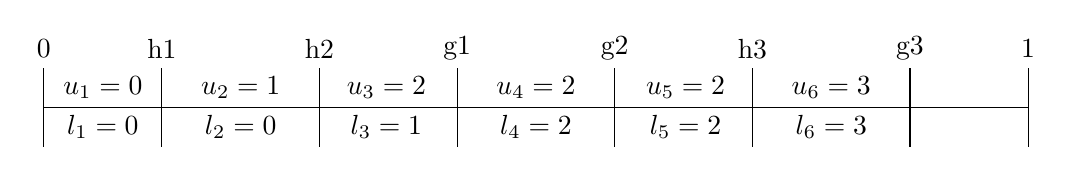
\begin{tikzpicture}
\draw (0,0) --(12.5,0);
\draw (0,-.5) --(0,.5);
\node at (0,.75) {0};
\draw (12.5,-.5) --(12.5,.5);
\node at (12.5,.75) {1};
\draw (1.5,-.5) --(1.5,.5);
\node at (1.5,.75) {h1};
\draw (5.25,-.5) --(5.25,.5);
\node at (5.25,.75) {g1};
\draw (9,-.5) --(9,.5);
\node at (9,.75) {h3};
\draw (3.5,-.5) --(3.5,.5);
\node at (3.5,.75) {h2};
\draw (7.25,-.5) --(7.25,.5);
\node at (7.25,.75) {g2};
\draw (11,-.5) --(11,.5);
\node at (11,.75) {g3};
\node at (.75,.25) {$u_{1} = 0$};
\node at (.75,-.25) {$l_{1} = 0$};
\node at (2.5,.25) {$u_{2} = 1$};
\node at (2.5,-.25) {$l_{2} = 0$};
\node at (4.35,.25) {$u_{3} = 2$};
\node at (4.35,-.25) {$l_{3} = 1$};
\node at (6.25,.25) {$u_{4} = 2$};
\node at (6.25,-.25) {$l_{4} = 2$};
\node at (8.15,.25) {$u_{5} = 2$};
\node at (8.15,-.25) {$l_{5} = 2$};
\node at (10,.25) {$u_{6} = 3$};
\node at (10,-.25) {$l_{6} = 3$};
\end{tikzpicture}
\caption{Example of how $l_{k}$ and $u_{k}$, $k = 1, ..., 2n$, depend on the relative positions of $h_{1}, ..., h_{n}$ and $g_{1}, ..., g_{n}$, for a case with n = 3. }
\end{figure}
Finally, we define
%
\begin{equation*}
    c_{w}^{(k)} = P_{0}(S_{k} = w \textrm{ and } l_{j} \leq S_{j} \leq u_{j} \textrm{ for } j = 1, ..., k - 1), \textrm{for } k = 1, ..., 2n \textrm{ and } w = 1, ..., n.
\end{equation*}
%
Our basic approach to step 1 is a recursive calculation of these $c_{w}^{(k)}$ values. Then, the global level $\alpha$ could be computed as $1 - c_{n}^{(2n)}$ in the general case. However, for the special case in which $(h_{1}, g_{1}), ..., (h_{n}, g_{n})$ are derived from equal local levels, i.e. equation (2) holds, then as a result of the symmetry in the problem, we need only calculate $c_{w}^{(k)}$ for $k = 1, ..., n+1$ instead of $k = 1, ... , 2n$. This shortcut is implemented below in the pseudocode for step 1. The algorithm calculates the probability of a valid allocation (under the null hypothesis) of points in bins by looping over each bin and making a recursive calculation.
% In this algorithm I think that I want to introduce Mary Sara's calculation. I should maybe introduce some notation before this, but I think that it's probably fine.
\begin{algorithm}[H]
\caption{Calculate Type I error $\alpha$ from proposed rejection region}
\textbf{Input:} Vector of lower bound values $(h_{1}, ..., h_{n})$, vector of upper bound values $(g_{1}, ..., g_{n})$, where we require $h_{i} < g_{i}$ for $i = 1, ..., n$.
\newline
\textit{get\_level\_from\_bounds\_two\_sided}$(h_{1}, ..., h_{n}, g_{1}, ..., g_{n})$
\begin{algorithmic}[1]
\STATE $b_{1}, ..., b_{2n} \leftarrow \textbf{sort}(h_{1}, ..., h_{n}, g_{1}, ..., g_{n})$
\STATE {$c_{0}^{(1)} \leftarrow (1 - b_{1})^{n}$}
\STATE $l_{k} \leftarrow 0$
\STATE $u_{k} \leftarrow 0$
\FOR{$k = 2, ..., n + 1$}
\IF{$b_{k - 1} \in \{h_{1}, ..., h_{n}\}$}
\STATE $u_{k} \leftarrow u_{k - 1} + 1$
\ENDIF
\IF{$b_{k} \in \{g_{1}, ..., g_{n}\}$}
\STATE $l_{k} \leftarrow l_{k - 1} + 1$
\ENDIF
\FOR{$j = l_{k}, ..., u_{k}$}
\STATE $c_{j}^{(k)} \leftarrow 0 $
\FOR{$m = l_{k - 1}, ..., min(u_{k - 1}, j)$}
\STATE $c_{j}^{(k)} \leftarrow  c_{j}^{(k)} + c_{m}^{(k - 1)} * dbinom(x = j - m, size = n-m, prob = \frac{(b_{k} - b_{k - 1})}{(1 - b_{k - 1})})$
\ENDFOR
\ENDFOR
\ENDFOR
\STATE $1 - \alpha \leftarrow 0$
\FOR{$l = l_{n}, ..., u_{n}$}
\STATE $1 - \alpha \leftarrow 1 - \alpha + \frac{c_{l}^{(n)} * c_{n - l}^{(n + 1)}}{dbinom(x = l, size = n, prob = b_{n})}$
\ENDFOR
\RETURN $\alpha$
\end{algorithmic}
\textbf{end}
\end{algorithm}
% Note, need to change all of the l values below to m's to match what the algorithm says above
% Also need to finish writing out the algorithm
% I can do all of this either tonight or tomorrow at some point
% Then I also need to get the bibliography and to the pre-computation for the graphs.
Now, we derive the algorithm. \textbf{Initialization:} (Lines 2 through 4 of Algorithm 1)
%
\begin{align*}
    c_{0}^{(1)} &= P_{0}(S_{1} = 0)\\
    &= P_{0}\Big(\bigcap\limits_{i=1}^{n}\{X_{i} \in (b_{1}, 1)\}\Big)\\
    &= \prod\limits_{i=1}^{n}P_{0}\Big(X_{i} \in (b_{1}, 1)\Big) &\textrm{(by independence)}\\
    &= (1 - b_{1})^{n} &\textrm{(Since each $X_{i} \sim~ U(0, 1)$ under the null)}
\end{align*}
%
Also, we initialize $l_{1} = 0$ and $u_{1} = 0$ because the only allowable partial sum is 0 in the first bin.
\textbf{Recursion:} (Line 15 of Algorithm 1)
%
\begin{flalign*}
    \indent\indent c_{j}^{(k)} &= P_{0}(S_{k} = j \textrm{ and } l_{q} \leq S_{q} \leq u_{q} \textrm{ for } q = 1, ..., k - 1)\\
    &= P_{0}\Big(\bigcup\limits_{m=l_{k- 1}}^{min(j, u_{k- 1})} \{S_{k - 1} = m \textrm{ and } N_{k} = j - m \textrm{ and } l_{q} \leq S_{q} \leq u_{q} \textrm{ for } q = 1, ..., k - 2\}\Big)\\
    &= \sum\limits_{m=l_{k- 1}}^{min(j, u_{k- 1})}P_{0}(S_{k - 1} = m \textrm{ and } N_{k} = j - m \textrm{ and } l_{q} \leq S_{q} \leq u_{q} \textrm{ for } q = 1, ..., k - 2)\\
    &= \sum\limits_{m=l_{k- 1}}^{min(j, u_{k- 1})}P_{0}(S_{k - 1} = m \textrm{ and } l_{q} \leq S_{q} \leq u_{q} \textrm{ for } q = 1, ..., k - 2)*\\
    &P_{0}(N_{k} = j - m | S_{k - 1} = m \textrm{ and } l_{q} \leq S_{q} \leq u_{q} \textrm{ for } q = 1, ..., k - 2)\\
    &= \sum\limits_{m=l_{k- 1}}^{min(j, u_{k- 1})}c_{m}^{(k - 1)} * P_{0}(N_{k} = j - m | S_{k - 1} = m)\\
    &= \sum\limits_{m=l_{k- 1}}^{min(j, u_{k- 1})}c_{m}^{(k - 1)} * P(B = j - m), \textrm{where }B \sim Binomial\left(n - m, \frac{b_{k} - b_{k - 1}}{1 - b_{k - 1}}\right),
    &&
\end{flalign*}
%
\newline
\indent\indent which is easily computed.
\newline
\newline
As noted above, in the general case, we could use this recursion to obtain $c_{n}^{(2n)}$, and then compute $\alpha = 1 - c_{n}^{(2n)}$. However, in the special case of equal local levels, we can use symmetry to speed the calculation by only computing the $c_{w}^{(k)}$ values for $k = 1, ..., n+1$ and $w = 1, ..., n$, and performing the calculation on line 21 of Algorithm 1, as we now demonstrate. First, we define the following values:
%
\begin{align*}
\Tilde{u}_{k} &=
    \begin{cases}
      0, & \text{if}\ k = 2n \\
      \sum_{i = k + 1}^{2n} \mathds{1} \big(b_{i} \in \{g_{1}, ..., g_{n}\}\big), & \text{otherwise}
    \end{cases}\\
    \Tilde{l}_{k} &=
      \sum_{i = k}^{2n} \mathds{1} \big(b_{i} \in \{h_{1}, ..., h_{n}\}\big)\\
    T_{k} &= \sum_{j = k + 1}^{2n + 1}N_{j} = n - S_{k}
\end{align*}
%
Now, we make the following observations:
\newline
\newline
(1) With equal local levels, $g_{i} = 1 - h_{n + 1 - i}$ for $i = 1, ..., n$ since $F_{Beta(i, n + 1 - i)}^{-1}(1 - \frac{\eta}{2})$ = $1 - F_{Beta(n + 1 - i, i)}^{-1}(\frac{\eta}{2})$.
\newline
\newline
(2) $b_{k} = 1 - b_{2n + 1 - k}$ for $k = 1, ..., 2n$ by (1). 
\newline
\newline
(3) $u_{k} = \Tilde{u}_{2n + 1 - k}$ and $l_{k} = \Tilde{l}_{2n + 1 - k}$, for $k = 1,..., 2n$ by (1) and (2).
\newline
\newline
(4) The random vector $(N_{1}, ..., N_{k})$ has the same distribution as $(N_{2n + 1}, ..., N_{2n+2-k})$ for $k = 1, ..., 2n + 1$. This follows from the fact that the vector $(X_{1}, ..., X_{n})$ has the same distribution as $(1 - X_{1}, ..., 1 - X_{n})$ (since each $X_{i}$ is independent uniform) and (2).
\newline
\newline
(5) The random vector $(S_{1}, ..., S_{k})$ has the same distribution as $(T_{2n}, ..., T_{2n + 1 - k})$ for $k = 1, ..., 2n$. This follows from (4). 
\newline
\newline
(6)
%
\begin{align*}
    c_{j}^{(k)} &= P_{0}(S_{k} = j \textrm{ and } l_{q} \leq S_{q} \leq u_{q} \textrm{ for } q = 1, ..., k - 1)\\
    &= P_{0}(T_{2n + 1 - k} = j \textrm{ and } \Tilde{l}_{r} \leq T_{r} \leq \Tilde{u}_{r} \textrm{ for } r = 2n + 2 - k, ..., 2n).\\
\end{align*}
%
This follows from (3) and (5). 
\newline
\newline
(7) Conditional on $S_{k}$, the random vector $(X_{(S_{k} + 1)}, ..., X_{(n)})$ is distributed as the order statistics of $n - S_{k}$ $U(b_{k}, 1)$ independent random variables.
\newline
\newline
(8) The random vector $(S_{1}, ..., S_{r})$ and the random vector $(T_{r}, ..., T_{n})$ are independent conditional on $S_{r}$. This follows directly from (7).
\newline
\newline
Combining the above results, we can write
%
\begin{equation*}
    \{X_{(i)} \in (h_{i}, g_{i}) \textrm{ for } i = 1,..., n\} = \{l_{k} \leq S_{k} \leq u_{k} \textrm{ for } k = 1, ..., 2n\}
\end{equation*}
%
Also, observe that for any $2 \leq r \leq 2n - 1$, we have
%
\begin{equation*}
    \{l_{k} \leq S_{k} \leq u_{k} \textrm{ for } k = 1, ..., 2n\} = 
\end{equation*}
%
\begin{equation*}
    \{l_{k} \leq S_{k} \leq u_{k} \textrm{ for } k = 1, ..., r \textrm{ and } T_{r} = n - S_{r} \textrm{ and } \Tilde{l}_{k} \leq T_{q} \leq \Tilde{u}_{k} \textrm{ for } q = r, ..., 2n\}
\end{equation*}
%
Thus, we can write 
%
\begin{align*}
    \sum_{j = l_{r}}^{u_{r}} &P(S_{r} = j \textrm{ and } l_{k} \leq S_{k} \leq u_{k} \textrm{ for } k = 1, ..., r - 1)\\
    &\cdot I(\Tilde{l}_{r} \leq n - j \leq \Tilde{u}_{r})
    \cdot P(\Tilde{l}_{q} \leq T_{q} \leq \Tilde{u}_{r} \textrm{ for } q = r + 1,..., 2n | T_{r} = n - j)\\
    &= \sum_{j = l_{r}}^{u_{r}} c_{j}^{(r)} \cdot I(\Tilde{l}_{r} \leq n - j \leq \Tilde{u}_{r}) \cdot P(\Tilde{l}_{q} \leq T_{q} \leq \Tilde{u}_{r} \textrm{ for } q = r + 1,..., 2n | T_{r} = n - j) \\
    &= \sum_{j = l_{r}}^{u_{r}} c_{j}^{(r)} \cdot I(\Tilde{l}_{r} \leq n - j \leq \Tilde{u}_{r}) \cdot \frac{P(\Tilde{l}_{q} \leq T_{q} \leq \Tilde{u}_{r} \textrm{ for } q = r + 1,..., 2n \textrm{ and } T_{r} = n - j)}{T_{r} = n - j} \\
    &= \sum_{j = l_{r}}^{u_{r}} c_{j}^{(r)} \cdot \frac{c_{n - j}^{(2n + 1 - r)}}{\binom{n}{j}b_{r}^{j}(1 - b_{r})^{n-j}}
\end{align*}
%
Now, if we let $r = n$ above, then we get 
%
\begin{equation*}
    P_{0}\Big(\bigcap\limits_{i=1}^{n} X_{(i)} \in (h_{i}, g_{i})\Big) = \sum_{j = l_{n}}^{u_{n}} c_{j}^{(n)} \cdot \frac{c_{n - j}^{(n + 1)}}{\binom{n}{j}b_{n}^{j}(1 - b_{n})^{n-j}}
\end{equation*}
%
which is line 21 in the psuedo-code above.
\newline
\newline
Empirically, it seems that our algorithm has computational complexity $O(n^{2})$. For a dense grid of values of $n$ between $10$ and $50,000$, the number of recursive steps required (line 15 in algorithm 1 above) scales with $n^{2}$. More precisely, it appears that the number of recursive steps required is very close to $8n^{2}$. While each recursive step itself requires calculating a binomial probability which is $O(n)$ due to the calculation of the binomial coefficient multiplied by a quantity with powers as large as $n$, these calculations can be memoized with $O(n^{2})$ cost. Thus, these binomial probability calculations do not change the big $O$ complexity of the algorithm.
\newline
\newline
% The step below should definitely be put in an algorithm float as well. I need to make sure all of this makes sense before I finish it, but afterh this the discussion and the abstract should be relatively easy to follow through on and complete.
\textbf{Step 2:} This step is done with a simple binary search over $\eta$. We begin by setting $\eta_{upper} = \frac{-log(1 - \alpha)}{(2 * log(log(n)) * log(n))}$ since this is an upper bound on the local level as shown by Gontscharuk et al., and we set $\eta_{lower} = \frac{\alpha}{n}$, as this is the lower bound given by the Bonferroni correction. The pseudocode is shown below:
\begin{algorithm}[H]
\caption{Calculate testing bounds from global level $\alpha$ and sample size $n$}
\textbf{Input:} Local level $\alpha$, sample size $n$, tolerance $\epsilon$
\newline
\textit{get\_bounds\_two\_sided}$(\alpha, n, \epsilon)$
\begin{algorithmic}[1]
\STATE $\eta_{upper} \leftarrow \frac{-log(1 - \alpha)}{(2 * log(log(n)) * log(n))}$
\STATE $\eta_{lower} \leftarrow \frac{\alpha}{n}$
\STATE $\alpha_{mid} \leftarrow \infty$
\WHILE{$\frac{\alpha_{mid} - \alpha}{\alpha} > \epsilon$}
\STATE $\eta_{mid} \leftarrow \frac{\eta_{upper} + \eta_{lower}}{2}$
\STATE $h_{1}, ..., h_{n} \leftarrow qbeta(p = \frac{\eta_{mid}}{2}$, shape1 = c(1:n), shape2 = c(n:1))
\STATE $g_{1}, ..., g_{n} \leftarrow qbeta(p = 1 - \frac{\eta_{mid}}{2}$, shape1 = c(1:n), shape2 = c(n:1))
\STATE $\alpha_{mid} \leftarrow get\_level\_from\_bounds\_two\_sided(h_{1}, ..., h_{n}, g_{1}, ..., g_{n})$
\ENDWHILE
\RETURN $h_{1}, ..., h_{n}, g_{1}, ..., g_{n}$
\end{algorithmic}
\textbf{end}
\end{algorithm}
\section{Local Level Approximations in Large Samples}
\label{sec:approx}
For sufficiently large values of the number of tests $n$, it can be expedient to apply an accurate asymptotic approximation of the local level $\eta$ corresponding to global level $\alpha$ in place of exact computation. Previously, Gontscharuk and Finner showed that the asymptotic local level for global level $\alpha$ and number of tests $n$ is
%
\begin{equation*}
    \eta_{asymp} = \frac{log(1 - \alpha)}{2log(log(n))log(n)}
\end{equation*}
%
\citep{gontscharuk2017asymptotics}. However, as they note, this approximation gives poor performance for $n$ even as large as $10^{4}$. To improve this approximation, they propose to add a smaller order correction term, resulting in an approximation of the form
%
\begin{equation}
    \eta_{approx} = \frac{log(1 - \alpha)}{2log(log(n))log(n)}\left[1 - c_{\alpha}\frac{log(log(log(n)))}{log(log(n))}\right],
\end{equation}
%
where $c_{\alpha}$ is chosen empirically. For the values $\alpha = .01, .05, \textrm{ and } .1$ they chose $c_{\alpha} = 1.6, 1.3, \textrm{ and } 1.1$, respectively. To select these $c_{\alpha}$ values, the authors calculated the values of $\eta$ to high precision on a grid of values up until $n = 10,000$. To further test these approximations, we decided to calculate the values of $\eta$ with high precision on a grid of values up to $n = 500,000$ for $\alpha = .01, .05$. Based on our evaluation, we found that $c_{\alpha} = 1.3$ is satisfactory for $\alpha = .05$, but that $c_{\alpha} = 1.6$ for $\alpha = .01$ was not sufficiently accurate for our purposes (see Figure 2).
\begin{figure}
\begin{center}
    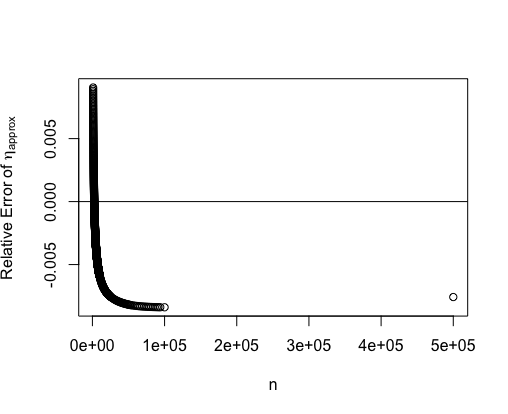
\includegraphics{images/c_alpha_1_6.png}
    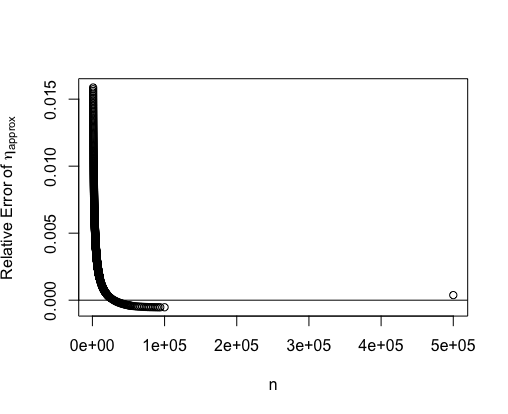
\includegraphics{images/c_alpha_1_591.png}
\end{center}
\caption{Relative Error of Local Level vs. Number of Tests for $\eta_{approx}$ for $\alpha = .01$ with $c_{\alpha} = 1.6$ (top) $c_{\alpha} = 1.591$ (bottom).}
\end{figure}
This approximation begins anti-conservative for small values of $n$, becomes very accurate for values of $n$ around 2,500, and then becomes and remains substantially conservative for even very large values of $n$. 
\newline
\newline
In addition to implementing algorithms 1 and 2, which, in principle, can be applied for any $n$ and $\alpha$, our package offers a faster approximate approach specifically for $\alpha = .01 \textrm{ and } .05$. For smaller values of $n$, up to $100,000$, we have pre-calculated values of $\eta$ on a dense grid of values of $n$. If the user inputs a value of $n$ less than or equal to $100,000$, we either return back the pre-computed value of $\eta$ if $n$ happens to be a grid point, or we use linear interpolation if the value of $n$ is between grid points, which leads to a highly accurate approximation. If the user inputs a value of $n$ greater than $100,000$, we use the asymptotic approximation given in (3), but with $c_{\alpha} = 1.591 \textrm{ and } 1.3$ for $\alpha = .01 \textrm{ and } .05$, respectively. We found that $c_{\alpha} = 1.591$ led to much better performance for $\alpha = .01$ for large values of $n$, as can be seen in Figure 2. Our package also implements the approximation given in equation (3) for $\alpha = .1$ with $c_{\alpha} = 1.1$, but we did not pre-compute any grid for these values due to limited computational resources.
\section{Examples}
\label{sec:examples}
As noted above, the algorithm presented is suitable for the case when all of the parameters of $F_{0}$ are known, and all $X_{1}, ..., X_{n}$ are independent. While these assumptions may seem restrictive, the methods above are still useful in a variety of scenarios.
\newline
\newline
One of the main advantages of the local levels method compared to other global testing approaches, is that it can easily be used to put testing bands onto Q-Q plots by simply graphing each $(h_{i}, g_{i})$ interval. This allows us to examine how a dataset might deviate from some null distribution much better than simply applying a test that yields a binary conclusion. Below, we present a few examples where a Q-Q plot is useful, and where the local levels test seems ideal for assessing deviation from a global null hypothesis.

\subsection{Examining the P-value Distribution for Testing Procedures}

% It may also make sense for me to make a comparison to the Kolmogorov-Smirnov statistic at some point. I should probably include some instructive graphs or something.
% I want to have a different paragraph to better introduce the concept
% This shouldn't be too difficult
Suppose we have devised a new testing procedure to test a null hypothesis $H_{0}$ with test statistic $T$, where we also specify a particular method to calculate or approximate p-values. In such a situation it is important to perform some simulations under the null hypothesis and check that the resulting p-value distribution is approximately uniform in the simulation experiment.
\newline
\newline
Typically, the verification of Type I error rate is done using the following procedure:
\newline
\newline
(1) Generate $n$ simulated datasets under $H_{0}$, and calculate $T$ for each siulated dataset to obtain $T_{1}, ..., T_{n}$.
\newline
\newline
(2) Select a value of $\alpha$, and for each of $T_{1}, ..., T_{n}$, determine whether the null hypothesis is rejected at level $\alpha$. Let $N_{\alpha}$ be the observed number of the $n$ tests that are rejected at level $\alpha$.
\newline
\newline
(3) Let $\alpha^{*}$ denote the true probability of rejection under the above procedure. Test the null hypothesis $H_{0}: \alpha^{*} = \alpha$ by applying, e.g., a z-test of proportions or an exact binomial test to the data $N_{\alpha}$.
\newline
\newline
While the above procedure provides reliable information about the Type I error calibration for one level of $\alpha$, it provides little information about the global calibration of p-values. Instead, we suggest the following procedure:
\newline
\newline
(1) As above.
\newline
\newline
(2) For each $T_{i}$, calculate the corresponding p-value, $p_{i}$, to obtain $p_{1}, ..., p_{n}$.
\newline
\newline
(3) Make a q-q plot comparing $p_{1}, ..., p_{n}$ to a $U(0, 1)$ distribution, and apply the local levels procedure to create simultaneous testing bands for the null hypothesis that $p_{1}, ..., p_{n} \distras{iid} U(0, 1)$.
\newline
\newline
This allows us to easily visualize the global calibration of the p-values with just one graph and diagnose any issues if they exist. In Step 3, one could use many different testing bands. However, in the calibration of p-values, we typically don't have the expectation that our p-values would be more likely to deviate from uniform in any particular region, and so it makes sense to use the local levels test because it is agnostic to the alternative distribution. Moreover, since it is generally most concerning if small p-values are not calibrated, i.e. those in the lower tail of the uniform distribution, the local levels test is preferable to the standard KS test because it is much more sensitive in the tails (Aldor-Noiman 2013).

\subsubsection{Chi-Square Test for Independence in a $2$ X $2$ Table}
We apply this approach to assess the calibration of p-values from the Pearson Chi-Square test for independence in a $2 \times 2$ table.  A well-known rule of thumb is that the chi-square test is appropriate as long as the expected cell count in each cell under the null hypothesis is at least 5.  We fix the cell probabilities under the null hypothesis and consider two different cases: in scenario 1, the sample size is $s=200$ and the rule of thumb holds, and scenario 2, the sample size is only $s=20$ and the rule of thumb does not hold.  We use the local levels approach to generate simultaneous testing bands to assess the calibration of the p-values from the Pearson Chi-Square test for these two scenarios.\\

More specifically, in each scenario, we randomly generate $n=1000$ $2 \times 2$ tables under the null hypothesis, where each table contains $s$ observations, with $s=200$ in scenario 1 and $s=20$ in scenario 2.  For each table, the $s$ observations are i.i.d.\ with probability $q_{i,j}$ of falling in cell $(i,j)$, for $i=0,1, j=0,1$, where $q_{1,1} = a*b$, $q_{1,0} = a*(1-b)$, $q_{0,1} = (1-a)*b$, and $q_{0,0} = (1-a)*(1-b)$, with a=.15 and b=.4.  For each table, let $X_{i,j}$ denote the observed count in cell $(i,j)$.  If any table has $X_{0,0}+X_{0,1} = 0$ or $= s$, we discard the table and draw a new one, because that would imply that one of the rows of the table is empty, in which case the Pearson Chi-Squared test statistic is not defined.  Similarly, if any table has $X_{0,0}+X_{1,0} = 0$ or $=s$, we discard the table and draw a new one. The code to do this is shown below:
%
\begin{Schunk}
\begin{Sinput}
R> set.seed(8675309)
R> # Generate contingency tables for variables as defined above
R> generate_contingency_tables <- function(n, s, a, b) {
+    
+    cell_probs <- c(a * b, a * (1 - b), b * (1 - a), (1 - b) * (1 - a))
+    num_sims <- 0
+    sim_mat <- matrix(NA, nrow = n, ncol = 4)
+    
+    # Generate n simulations and append the contingency tables to a matrix
+    while (num_sims < n) {
+      
+      proposed_sim <- t(rmultinom(n = 1, size = s, prob = cell_probs))
+      
+      # Check to make sure that the chi-square statistic will be defined
+      if (proposed_sim[, 1] + proposed_sim[, 2] != 0 && 
+          proposed_sim[, 1] + proposed_sim[, 3] != 0 &&
+          proposed_sim[, 3] + proposed_sim[, 4] != 0 &&
+          proposed_sim[, 4] + proposed_sim[, 2]) {
+        
+        num_sims <- num_sims + 1
+        sim_mat[num_sims, ] <- proposed_sim
+        
+      }
+      
+    }
+    
+    return(sim_mat)
+    
+  }
R> scenario_1 <- generate_contingency_tables(n = 1000, s = 200, a = .15, b = .4)
R> scenario_2 <- generate_contingency_tables(n = 1000, s = 20, a = .15, b = .4)
\end{Sinput}
\end{Schunk}
%

For each of the tables in the resulting sample, a Pearson chi-square test statistic is calculated as $T = \sum_{i=0}^1\sum_{j=0}^1 \frac{(X_{i,j}-q_{i,j})^2}{q_{i,j}}$, where $X_{i,j}$ is the observed count in cell $(i,j)$.  For each scenario, this results in $n=1000$ test statistics, $T_1, \ldots, T_n$, one for each table.  From these, we obtain $n=1000$ p-values, $p_1, \ldots, p_n$ by applying the $\chi^2_1$ approximation, i.e., $p_i = 1-F(T_i)$ for $i=1,\ldots, n$, where $F$ is taken to be the c.d.f. of the $\chi^2_1$ distribution. The code to do this is shown below:

%
\begin{Schunk}
\begin{Sinput}
R> # Compute Pearson Chi-Square Test p-values for Set of Contingency Tables
R> get_p_values_from_c_tables <- function(c_tables, s) {
+    
+    chisq_numerator <- (
+      (c_tables[, 1] * c_tables[, 4] - c_tables[, 2] * c_tables[, 3]) / s
+    ) ^ 2
+    chisq_denominator <- (c_tables[, 1] + c_tables[, 2]) * 
+      (c_tables[, 1] + c_tables[, 3]) * 
+      (c_tables[, 3] + c_tables[, 4]) * 
+      (c_tables[, 2] + c_tables[, 4]) / 
+      (s ^ 3)
+    chisq_stats_vec <- chisq_numerator / chisq_denominator
+    p_vals <- pchisq(q = chisq_stats_vec, df = 1, lower.tail = FALSE)
+    return(p_vals)
+    
+  }
R> pvals_scenario_1 <- get_p_values_from_c_tables(scenario_1, s = 200)
R> pvals_scenario_2 <- get_p_values_from_c_tables(scenario_2, s = 20)
\end{Sinput}
\end{Schunk}
%


Figure 3 shows the resulting Q-Q plots for scenarios 1 (in blue) and 2 (in red), where the 45$^{\mbox{\footnotesize o}}$ line is shown as well as the testing bands obtained from the equal local levels procedure for testing, at global level .05, the null hypothesis that $p_1, \ldots, p_n$ have the same distribution as $n$ i.i.d.\ draws from Unif(0,1).  

\begin{Schunk}
\begin{Sinput}
R> library(qqconf)
R> n <- 1000
R> bounds <- get_bounds_two_sided(alpha = .05, n = 1000)
R> # Plot 3: Q-Q plot of P-values from Chi-Squared Test
R> # for Independence in a 2 x 2 Table
R> 
R> 
R> qq_conf_plot(
+    obs = pvals_scenario_2,
+    distribution = qunif,
+    method = "ell",
+    alpha = .05,
+    points_params = list(col="red", type="l")
+  )
R> # Add the Q-Q plot for scenario 1.
R> lines(c(1:n) / (n + 1), sort(pvals_scenario_1), col = "blue")
R> legend(
+    "topleft", 
+    legend = c("s=20","s=200"), 
+    col = c("red","blue"), 
+    lty = 1
+  )
\end{Sinput}
\end{Schunk}

\begin{figure}
\begin{center}
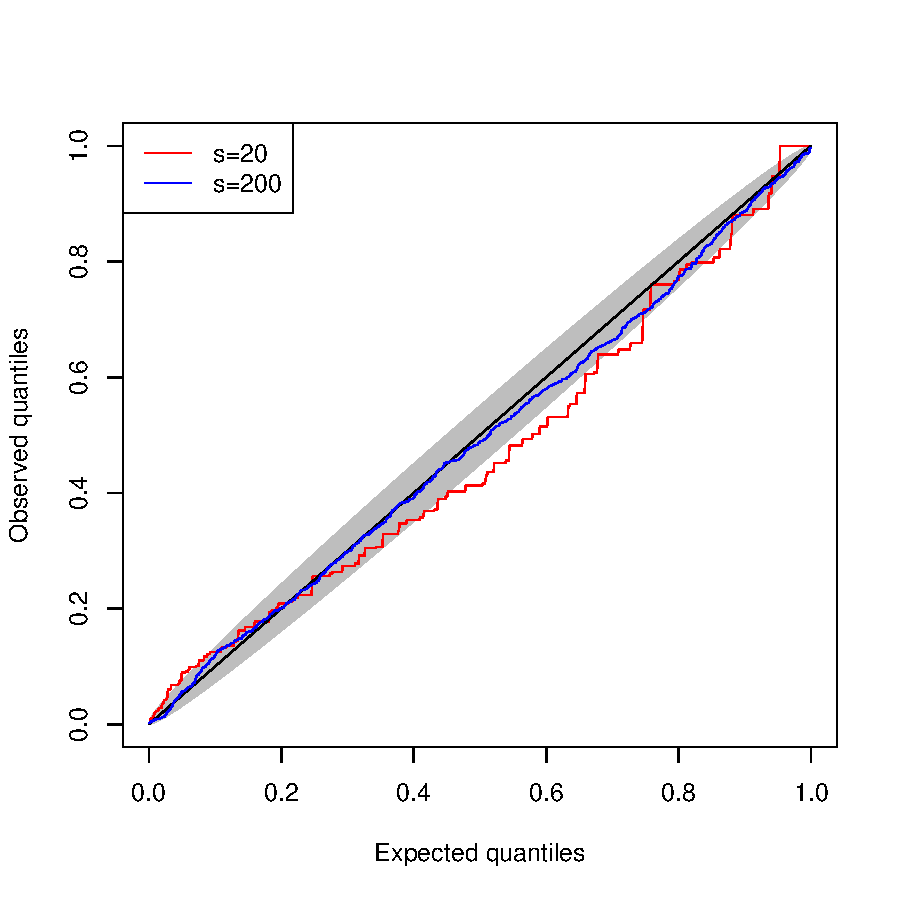
\includegraphics{manuscript-chisq_qq}
\end{center}
\caption{Q-Q plot for Scenario 1 and Scenario 2 With Standard Axes.}
\end{figure}

Figure 4 shows the same plots where the axes are transformed to be on the $-\log_{10}$ scale to focus the plot on small p-values. (Note that in Figure 4, small p-values are to the top and right of the plot, so a curve that is too low is conservative, and too high is anti-conservative.)  

\begin{Schunk}
\begin{Sinput}
R> # Plot 4: Q-Q plot, on the -log10 Scale, of P-values 
R> # from Chi-Squared Test for Independence in a 2 x 2 Table
R> n <- 1000
R> qq_conf_plot(
+    obs = pvals_scenario_2,
+    distribution = qunif,
+    method = "ell",
+    alpha = .05,
+    points_params = list(col="red", type="l"),
+    log10 = TRUE
+  )
R> # Add the Q-Q plot for scenario 1.
R> lines(-log10(c(1:n) / (n + 1)), -log10(sort(pvals_scenario_1)), col = "blue")
R> legend(
+    "topleft",
+    legend = c("s=20","s=200"), 
+    col = c("red","blue"), 
+    lty = 1
+  )
\end{Sinput}
\end{Schunk}

\begin{figure}
\begin{center}
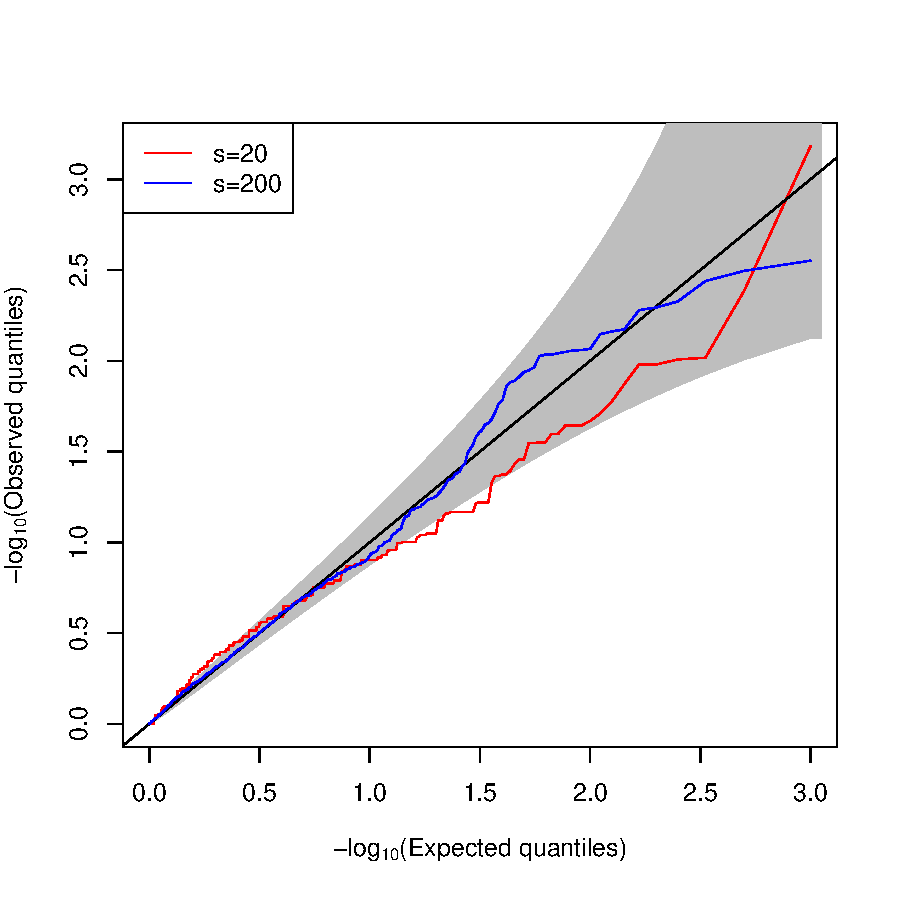
\includegraphics{manuscript-chisq_qq_log}
\end{center}
\caption{Q-Q plot for Scenario 1 and Scenario 2 With Axes On Log Scale.}
\end{figure}

From these plots, it can be seen that in scenario 1, when $s=200$ and the smallest expected cell count is 12, there is no significant deviation of the p-values from i.i.d.\ Unif(0,1) under the null hypothesis.  In contrast, in scenario 2, when $s=20$ and the smallest expected cell count is 1.2, the $\chi^2_1$ asymptotic distribution is not an accurate approximation to the sampling distribution of $T$.  As a result, we can see in Figures 3 and 4 that the p-values differ significantly from i.i.d.\ Unif(0,1) under the null hypothesis, with small p-values tending to be overly conservative, while the larger p-values tend to be anti-conservative.

\subsection{Testing for Normality of Regression Residuals}
When performing an ordinary least squares regression (OLS), it is common to assume that the error terms are idependentally drawn from a normal distribution. Specifically, suppose that we have $n$ observations $\{\mathbf{x_{i}}, y_{i}\}_{i=1}^{n}$, where each $y_{i}$ is a scalar and each $\mathbf{x_{i}}$ is a $1xp$ vector of regressors. Then, we model each $y_{i}$ as
\begin{equation*}
  y_{i} = \mathbf{x_{i}}^{T}\boldsymbol\beta + \epsilon_{i}
\end{equation*}
where $\mathbf{\boldsymbol\beta}$ is a $1xp$ vector of regression parameters to be estimated and we assume
\begin{equation}
  \epsilon_{1}, ..., \epsilon_{n} \distras{iid} N(0, \sigma^{2}).
\end{equation}
Once $\boldsymbol\beta$ and $\sigma^{2}$ are estimated (typically via maximum liklihood), for each $y_{i}$ we define the residual as 
\begin{equation*}
  r_{i} = \mathbf{x_{i}}^{T}\mathbf{\hat{\boldsymbol\beta}} - y_{i},
\end{equation*}
where $\hat{\boldsymbol\beta}$ is our estimate of $\boldsymbol\beta$. Then, we would like a Q-Q plot of the residuals with a Normal reference distribution to aid in testing assumption (4) above. Strictly speaking, even if assumption (4) is correct, the residuals are not independent because OLS leads to an estimation of $\hat{\boldsymbol\beta}$ such that $\sum_{i=1}^{n}r_{i} = 0$. However, accounting for the resulting negative correlation between the residuals when creating testing bands would be very difficult, and with a sufficiently large sample size this correlation becomes negligible. Thus, without an a priori reason to believe that the errors may deviate from normality at any particular point in the distribution, it makes sense to use ELL bands in this case. This is very easy to do with \pkg{qqconf}, as we show below.
\newline
\newline
First, we generate data to perform a regression. Here, we will generate each $\epsilon_{i}$ independently from a $t(2.5)$ distribution. 
%
\begin{Schunk}
\begin{Sinput}
R> set.seed(100)
R> n <- 100
R> x <- runif(n)
R> eta <- rt(n, df = 2.5)
R> y <- x + eta
\end{Sinput}
\end{Schunk}
%
Then, we fit a regression with the simulated data
%
\begin{Schunk}
\begin{Sinput}
R> reg <- lm(y ~ x)
\end{Sinput}
\end{Schunk}
%
With \pkg{base}-\proglang{R} functionality, we can can create a qqplot using the function \code{qqnorm} and \code{qqline}. 
%
%
\begin{Schunk}
\begin{Sinput}
R> qqnorm(reg$residuals)
R> qqline(reg$residuals)
\end{Sinput}
\end{Schunk}
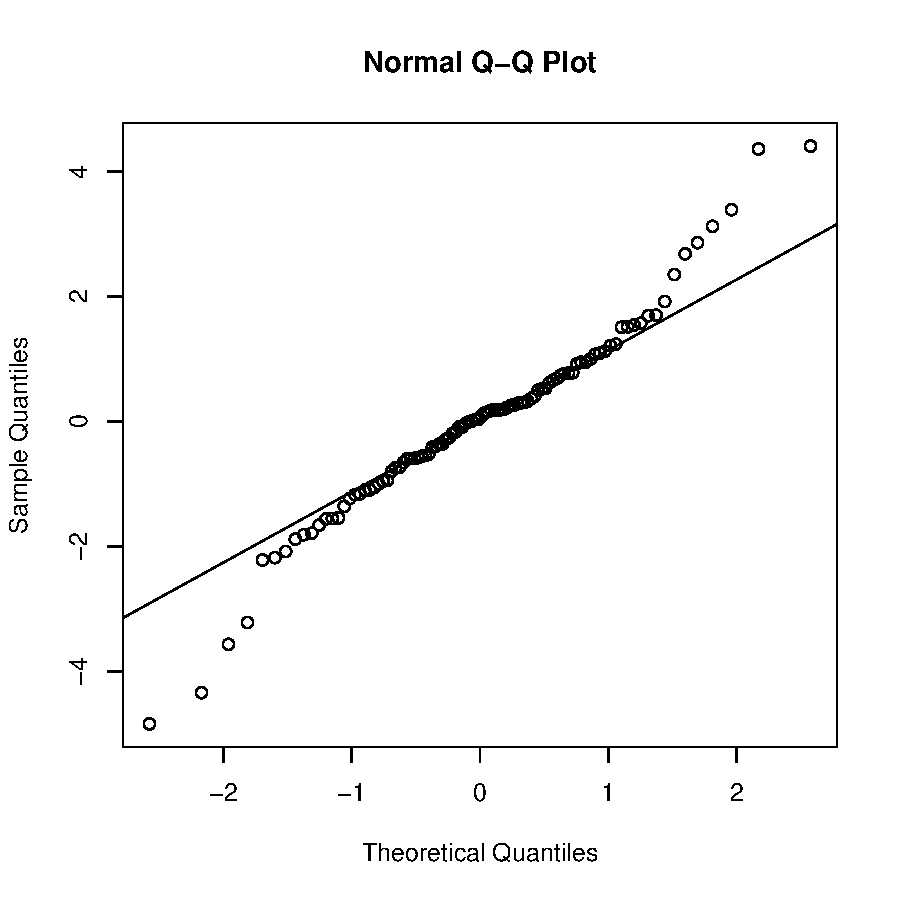
\includegraphics{manuscript-base_qqplot}
%
%
\newline
Clearly there's some indication of deviation in this plot, but it can be hard to tell how significant the deviation is without confidence bounds. With our function \code{qq_conf_plot}, it is much easier to be able to judge the significance of the deviation.
%
%
\begin{Schunk}
\begin{Sinput}
R> library(qqconf)
R> qq_conf_plot(
+    obs = reg$residuals,
+    points_params = list(col="red")
+  )
\end{Sinput}
\end{Schunk}
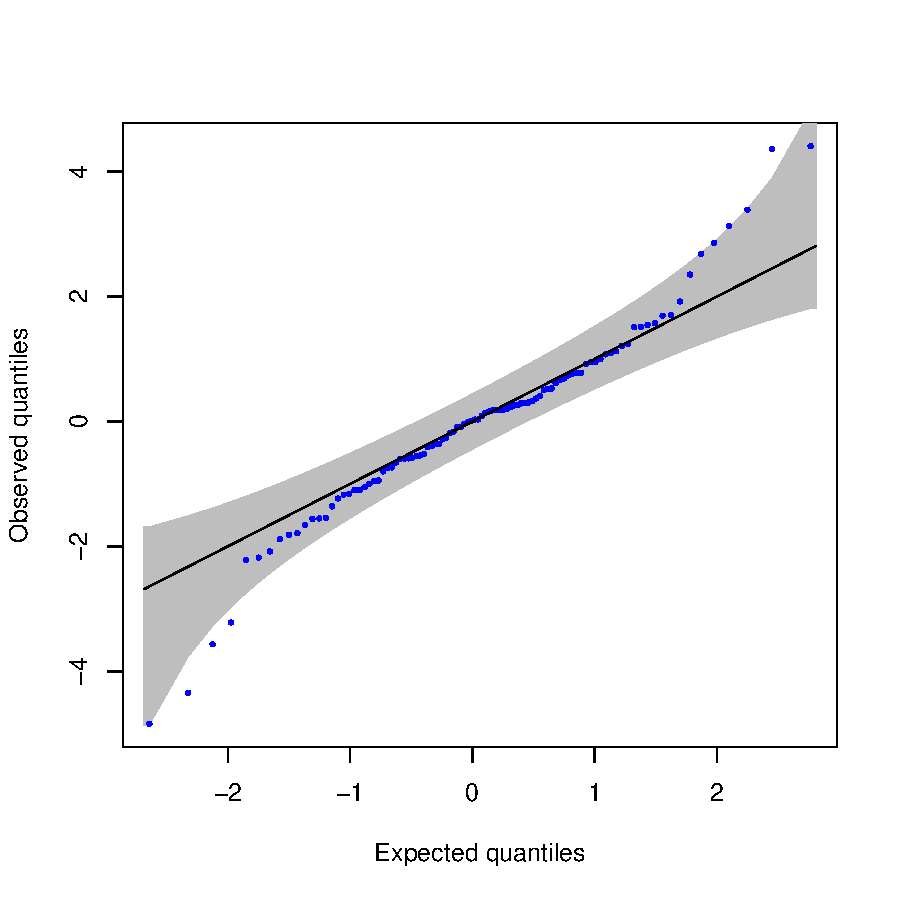
\includegraphics{manuscript-qqconf_qqplot}
%
%
\newline
Here, we can clearly see that in the right tail of the residuals goes beyond the normal testing bounds, giving strong evidence that the errors were not generated from a normal distribution. 

\subsection{Multiple Testing in Genome Wide Association Studies}
In genome wide association studies (GWAS), we are interested in identifying the genetic variants that are responsible for biological traits. Often, we test a large number of single-nucleotide polymorphisms (SNPs), to see if any of them are strongly correlated with some discrete or continuous trait. Often, it is useful to test the following global null hypothesis:
\newline
\newline
$H_{0}$: All genome-wide SNPs in some functional category have correlation 0 with the trait of interest.
%
\begin{equation*}
\textrm{ vs. }
\end{equation*}
%
\noindent$H_{A}$: At least one SNP in some functional category has non-zero correlation with the trait of interest.
\newline
\newline
Typically, when testing this global null, we apply some test to each of $n$ SNPs, yielding $n$ p-values. While the SNPs have a local correlation structure, this has only a weak effect at a genome-wide scale. Thus, the local levels procedure still provides a valuable visualization tool to assess the extent and type of any deviation from the null, even though it is not exact. Particularly in genetics, if the p-values deviate from the null, it can be very useful to view graphically how they deviate. For instance, if there are a few very large p-values but the rest of the distribution looks relatively uniform, then this indicates that the trait of interest is driven by a few mutations. If, however, there are some small deviations throughout the p-value distribution, then this indicates that trait of interest is driven by a number of genes that all play some small part in a complex biological process, or potentially by some confounding variables that are not controlled for.
\newline
\newline
If a very specific distribution for $H_{A}$ is suspected, then it makes sense to use a test that has high power under this alternative, which may not be our local levels test. However, in the general case when little is known about the alternative distribution, using local levels is desirable because it is agnostic to alternative distributions. Moreover, since small p-values are often of great interest in GWAS because they can indicate the main biological drivers of a trait, the local levels test is far superior to the KS test due to its tail sensitivity.
%Here is where the biological example goes with the code. I want to have the graphs that I make from this and then I also want
\section{Discussion}
\label{sec:discussion}
The local levels test using an exact recursive calculation allows for the creation of relatively fast and alternative-agnostic simultaneous testing bands for Q-Q plots. Of course, our method is limited by the assumptions that (1) all of the tests are independent and that (2) all of the parameters of the null distribution are known. Currently, we are not aware of methods to handle the dependent case that allow for bands on Q-Q plots. To handle the second issue, Aldor-Noiman has adapted their method such that it will yield exact results when some parameters of the null distribution are unknown. However, if the dataset is very large, Aldor-Noiman's method is prohibitively slow. In this case, we suggest that our method be used because it is much faster, and with a sufficiently large dataset the uncertainty in the parameters will become negligible under standard regularity conditions. Methods to handle parameter uncertainty with an exact calculation have been discussed in the context of the normal distribution \citep{rosenkrantz2000confidence}, but a general method towards this end has not been developed, and would be an important next step.
\newline
\newline
Our software is available on CRAN. To aid in computation speed, we have pre-computed a number of different local level values given a global level and the size of the dataset. This computes the testing bands very quickly with little error. We have also implemented a one-sided test for the case in which we are only concerned with values that are smaller than would be expected under the null (e.g. we only care about small p-values).

\bibliography{refs}
%\bibliographystyle{ieeetr}

\end{document}
